\section{Extra information on the PDAC analysis}
\label{appendix:clinical_covariates}
\raggedbottom


Although the main manuscript focuses on conditional treatment effects, we also report the average treatment effect (ATE) in the PDAC case study to facilitate comparison with existing clinical and methodological work. 
The ATE is defined as the population-level estimand:
\begin{equation}
\mathrm{ATE} := \E\!\left[\log T(1) - \log T(0)\right] = \E\left[\tau(x)\right],
\end{equation}
where the expectation is taken with respect to the covariate distribution in the target population.



We approximate this expectation by integrating the conditional average treatment effect over the empirical distribution of the observed covariates:
\begin{equation}
\widehat{\mathrm{ATE}}
= \frac{1}{n}\sum_{i=1}^n\widehat{\tau}(x_i).
\end{equation}
This plug-in estimator corresponds to averaging the posterior draws of the CATE over the observed covariate values and is standard in Bayesian tree-based causal models, including Bayesian causal
forests \citep{hahn2020bayesian}. 
The approach conditions on the observed covariates and therefore does not require specifying a probabilistic model for the covariate distribution.
This is also known as the MATE, or mixed average treatment effect \citep{Li2023BayesianCausal}.


Because the empirical covariate distribution is treated as fixed, this approximation does not explicitly propagate uncertainty in the covariate distribution itself.
More fully Bayesian alternatives, such as Bayesian bootstrap weighting of the covariate distribution, could be used to account for this additional source of uncertainty \citep{Oganisian2025Untangling}, but we do not
pursue these extensions here. 
Since our primary inferential focus is on heterogeneous treatment effects rather than average effects.




\begin{table}[H]
\centering
\label{tab:clinical_covariates}
% Changed 'll' to 'l p{9cm}' to allow text wrapping in the 2nd column
\begin{tabular}{l p{9cm}} 
\toprule
\textbf{Variable} & \textbf{Description} \\
\midrule
\multicolumn{2}{l}{\textit{Demographic information}} \\
\texttt{age} & Age of the patient at diagnosis (in years) \\
\texttt{sex} & Biological sex (0 = female, 1 = male) \\
\addlinespace % Better spacing than \\
\multicolumn{2}{l}{\textit{Tumor characteristics}} \\
\texttt{grade} & Histological tumor grade \\
\texttt{tumor.cellularity} & Tumor cellularity as estimated by pathologist (numeric) \\
\texttt{tumor.purity} & Estimated tumor purity (0 = low, 1 = high) \\
\texttt{absolute.purity} & Tumor purity estimated using ABSOLUTE algorithm (numeric) \\
\addlinespace
\multicolumn{2}{l}{\textit{Molecular and expression features}} \\
\texttt{moffitt.cluster} & Molecular subtype (0 = classical, 1 = basal-like) \\
\texttt{meth.leukocyte.percent} & Estimated leukocyte fraction based on DNA methylation (numeric) \\
\texttt{meth.purity.mode} & Tumor purity from methylation model (numeric) \\
\addlinespace
\multicolumn{2}{l}{\textit{Staging and metastasis}} \\
\texttt{stage} & Nodal stage (0 = N0: no regional nodes, 1 = N1: nodal metastasis) \\
\texttt{lymph.nodes} & Number of lymph nodes examined (numeric) \\
\bottomrule
\end{tabular}
\caption{Overview of clinical covariates used in the PDAC data analysis.}
\end{table}

\begin{table}[H]
\centering
\label{tab:literature_genes}
\begin{tabular}{lll}
\toprule
\textbf{Stefanoudakis et al. (2024)} & \textbf{Cicenas et al. (2017)} & \textbf{Takai \& Yachida (2015)} \\
\midrule
\textit{KRAS}    & \textit{BRCA1}    & \textit{ARID1A}  \\
\textit{TP53}    & \textit{BRCA2}    & \textit{ATM}     \\
\textit{CDKN2A}  & \textit{PALB2}    & \textit{RNF43}   \\
\textit{SMAD4}   &                   & \textit{KDM6A}   \\
                 &                   & \textit{PBRM1}   \\
                 &                   & \textit{MLL3} \\
                 &                   & \textit{ARID2}   \\
                 &                   & \textit{SF3B1}   \\
                 &                   & \textit{BRAF}    \\
                 &                   & \textit{NRG1}    \\
                 &                   & \textit{RET}     \\
\bottomrule
\end{tabular}
\caption{Genes identified as drivers in pancreatic ductal adenocarcinoma (PDAC) according to the literature.}
\end{table}

\begin{figure}[ht]
    \centering
    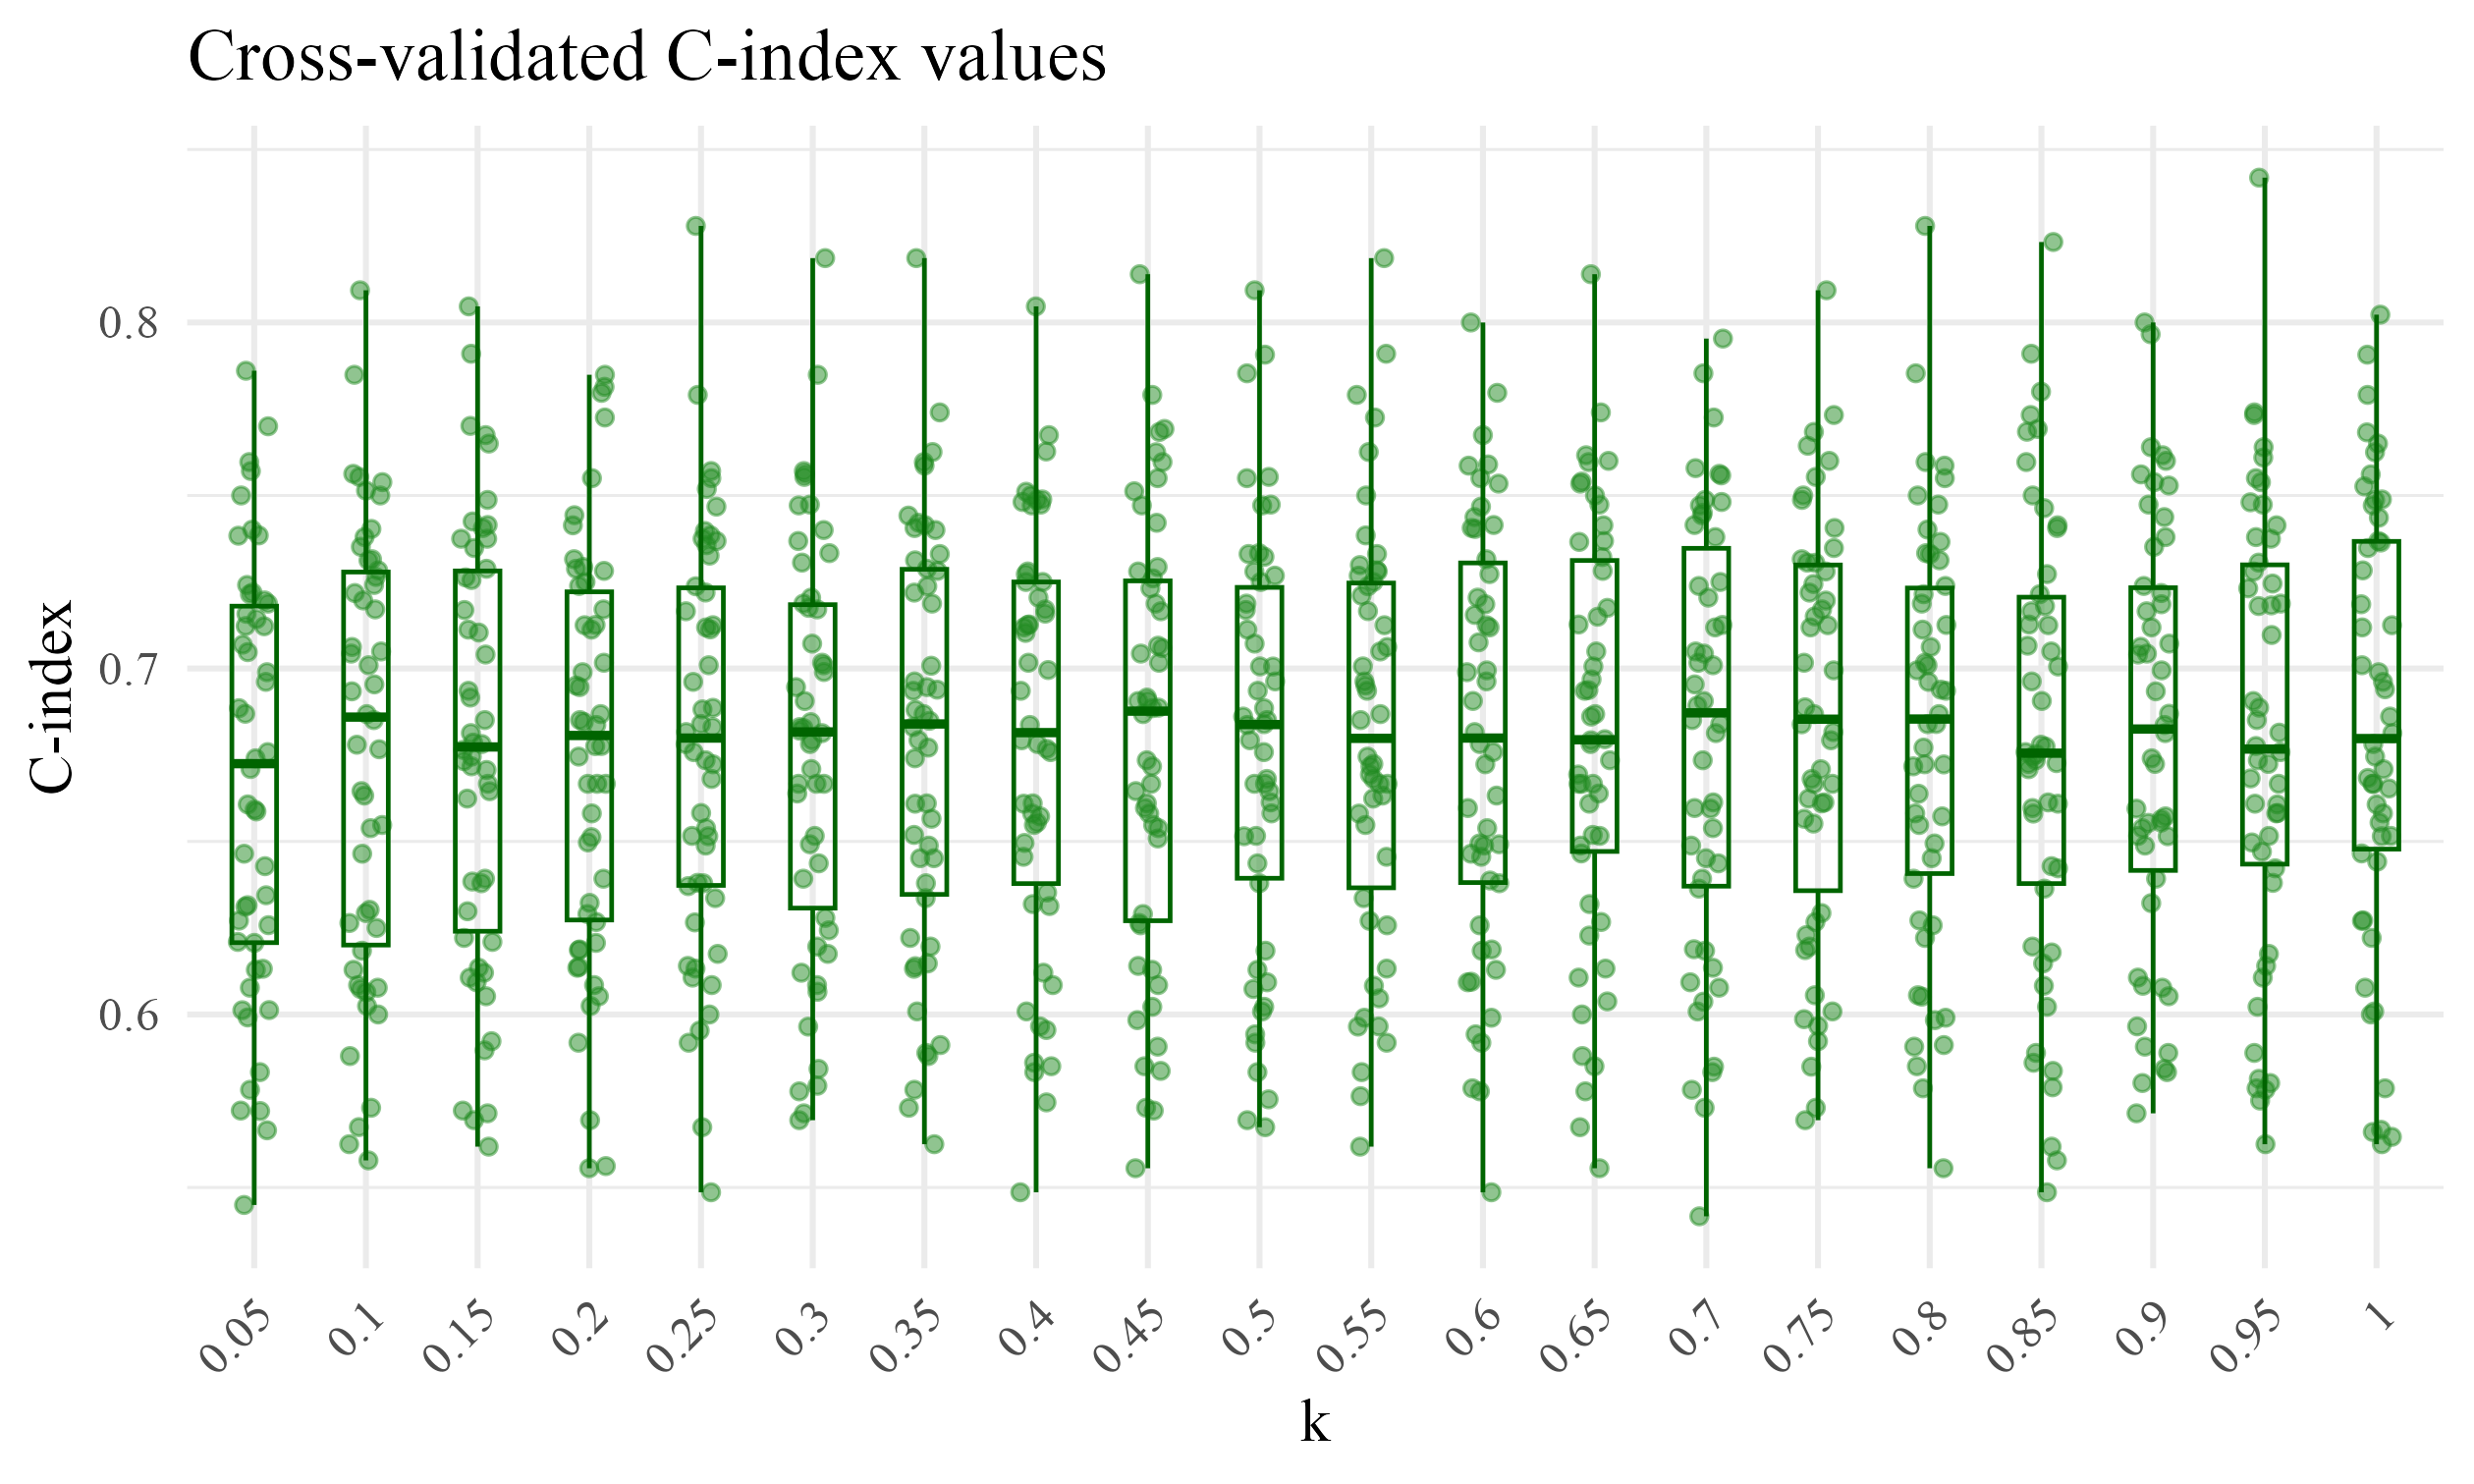
\includegraphics[width=0.9\linewidth]{cindex_crossval_omega05.png}
    \caption{Stratified $10 \times 5$ cross-validated C-index values across different shrinkage values $k$.}
    \label{fig:cindex_k}
\end{figure}

\begin{figure}[H]
    \centering
    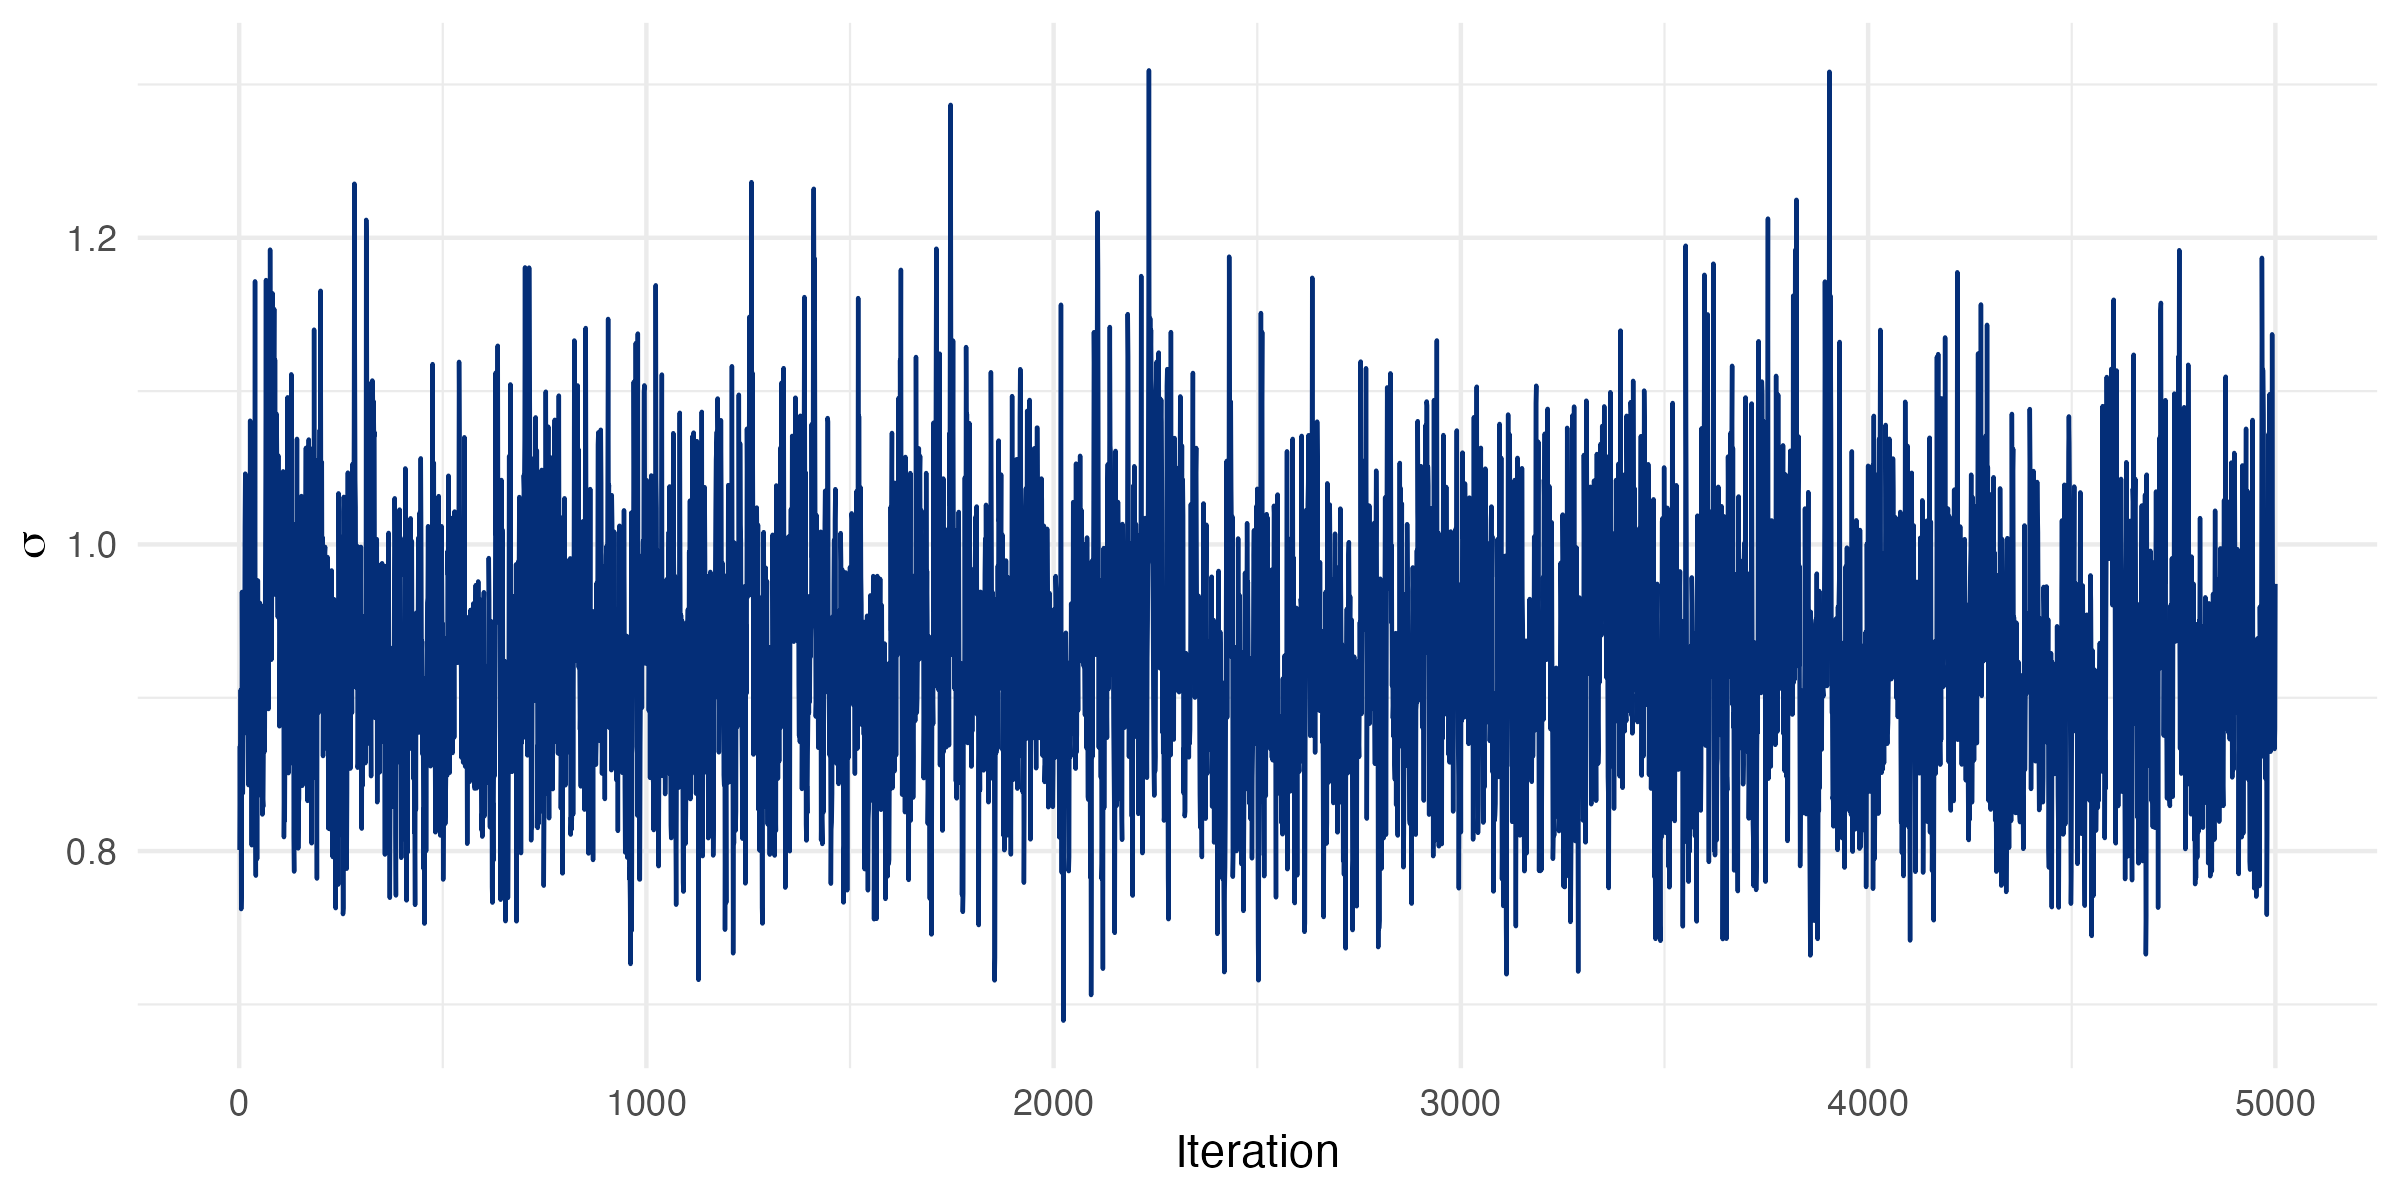
\includegraphics[width=\linewidth]{Traceplot_Sigma.png}
    \caption{Traceplot of the posterior samples of $\sigma$, used to assess convergence of the Causal Horseshoe Forest sampler.}
    \label{fig:traceplot_sigma}
\end{figure}

\begin{figure}[H]
    \centering
    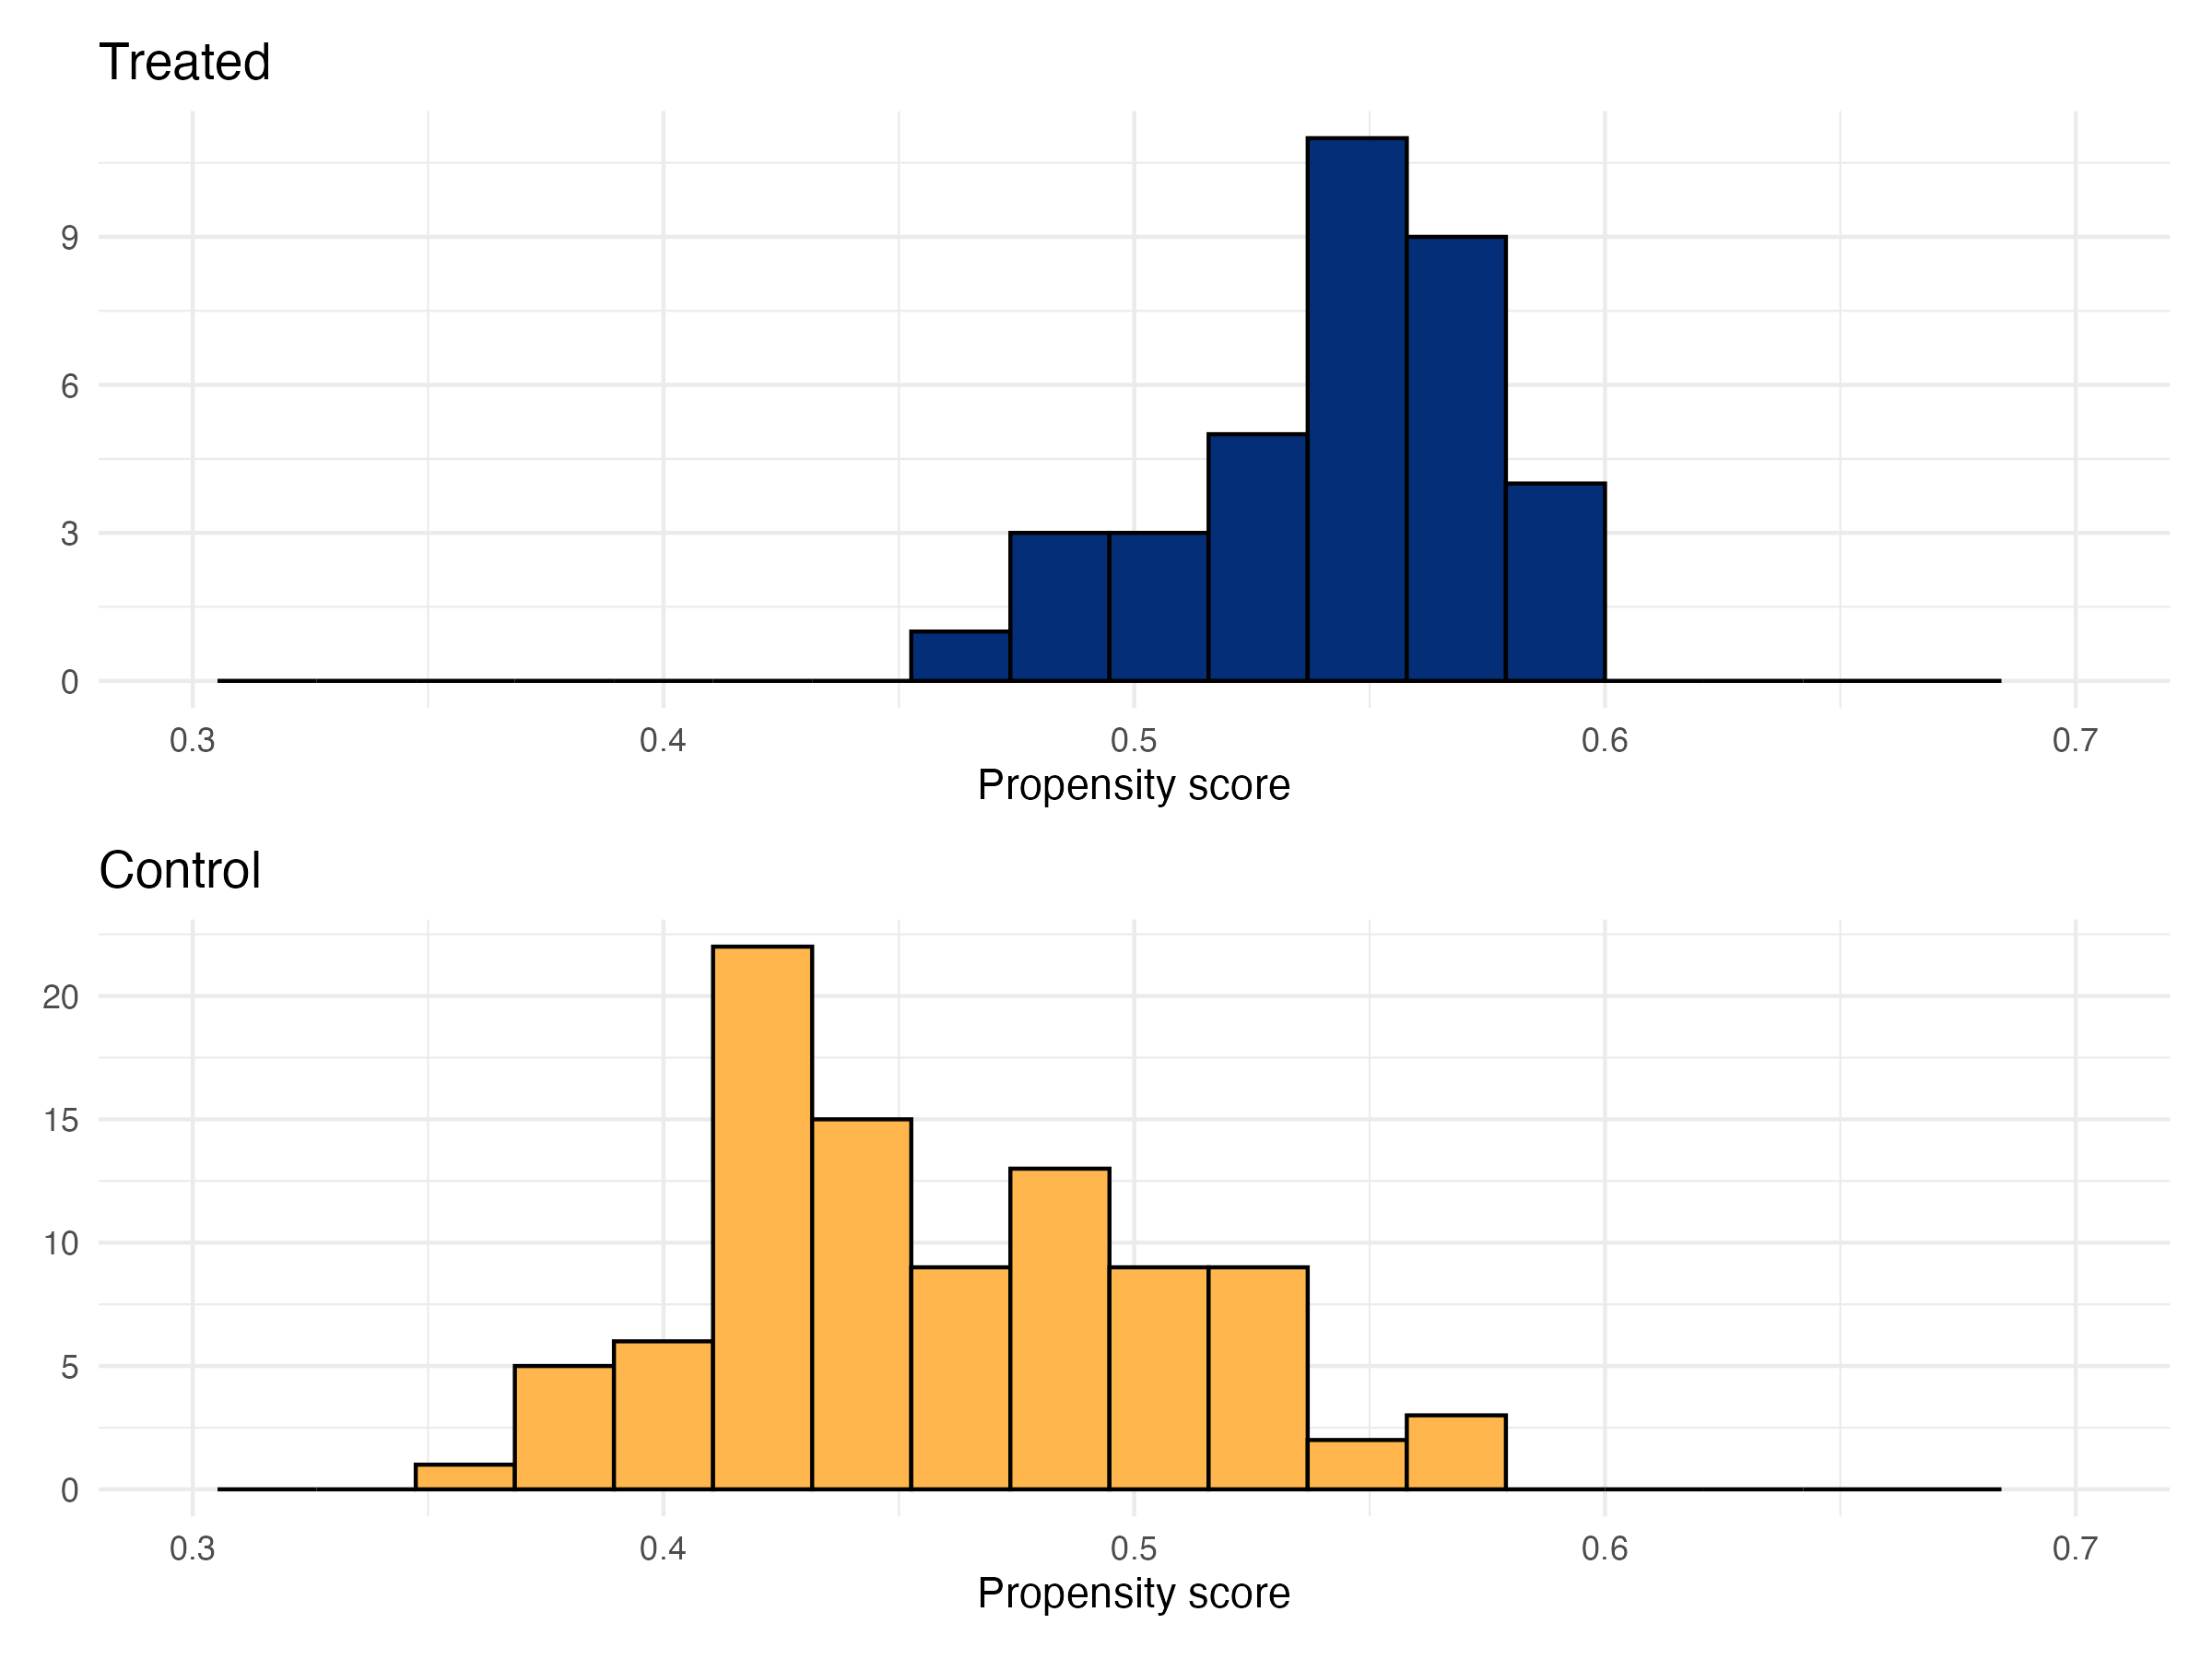
\includegraphics[width=0.9\linewidth]{Propensity_histograms.png}
    \caption{Histograms of estimated propensity scores for treated and control patients, showing the overlap in estimated treatment probabilities.}
    \label{fig:propensity_histograms}
\end{figure}

